%!TEX root = ../Thesis.tex
\chapter{Linear Time-Invariant Model}

\section{LTI System}

A discrete-time Linear Time-Invariant (LTI) system can be represented in state-space form as

\begin{align}
    x_{k+1} &= A x_k + B u_k, \label{eq:lti_state}\\
    y_k &= C x_k, \label{eq:lti_output}
\end{align}

where \(x_k \in \mathbb{R}^{n}\) denotes the state vector, 
\(u_k \in \mathbb{R}^{m}\) denotes the input vector, and 
\(y_k \in \mathbb{R}^{r}\) denotes the output vector at time step \(k\).
The matrices \(A\), \(B\), and \(C\) are the state, input, and output matrices, respectively.

For model predictive control, the future behavior of the system is predicted from the current state \(x_0\) and a sequence of future control inputs

\begin{equation}
    u_0,u_1,\ldots,u_{N-1},
\end{equation}

where \(N\) denotes the prediction horizon.

\subsection{State and Output Prediction}

Starting from the initial state \(x_0\), the state after one time step is obtained from \cref{eq:lti_state} as

\begin{equation}
    x_1 = A x_0 + B u_0
\end{equation}

At the next time step,

\begin{align}
    x_2
    &= A x_1 + B u_1 \\
    &= A(Ax_0 + Bu_0) + Bu_1 \\
    &= A^2x_0 + ABu_0 + Bu_1
\end{align}

Similarly, the third predicted state is

\begin{align}
    x_3
    &= Ax_2 + Bu_2 \\
    &= A^3x_0 + A^2Bu_0 + ABu_1 + Bu_2
\end{align}

Following the same recursion, the state at an arbitrary prediction step \(k\) can be written as

\begin{equation}
    x_k
    =
    A^k x_0
    +
    \sum_{i=0}^{k-1}
    A^{k-1-i}B u_i
    \label{eq:lti_xk}
\end{equation}

Equation~\cref{eq:lti_xk} separates the future state into two contributions. The first term represents the evolution of the initial state in the absence of future inputs, whereas the summation represents the contribution of the input sequence.

Using the output relation in \cref{eq:lti_output}, the corresponding output at prediction step \(k\) is

\begin{align}
    y_k
    &= Cx_k \\
    &= C
    \left(
        A^k x_0
        +
        \sum_{i=0}^{k-1}
        A^{k-1-i}Bu_i
    \right),
\end{align}

which gives

\begin{equation}
    y_k
    =
    CA^k x_0
    +
    \sum_{i=0}^{k-1}
    CA^{k-1-i}Bu_i
    \label{eq:lti_yk}
\end{equation}

Thus, each predicted output is expressed as a function of the current state and all control inputs applied before that prediction step.

\subsection{Stacked Prediction Formulation}

For optimization over a prediction horizon \(N\), the predicted outputs and future inputs can be collected into stacked vectors. The output vector is defined as

\begin{equation}
    Y =
    \begin{bmatrix}
        y_1 \\
        y_2 \\
        \vdots \\
        y_N
    \end{bmatrix}
    \in \mathbb{R}^{Nr},
    \label{eq:lti_Y}
\end{equation}

and the corresponding input vector is

\begin{equation}
    U =
    \begin{bmatrix}
        u_0 \\
        u_1 \\
        \vdots \\
        u_{N-1}
    \end{bmatrix}
    \in \mathbb{R}^{Nm}
    \label{eq:lti_U}
\end{equation}

The first two predicted outputs can be written explicitly as

\begin{align}
    y_1 &= CAx_0 + CBu_0, \\
    y_2 &= CA^2x_0 + CABu_0 + CBu_1,
\end{align}

and the final output over the prediction horizon is

\begin{equation}
    y_N
    =
    CA^N x_0
    +
    CA^{N-1}Bu_0
    +
    CA^{N-2}Bu_1
    +
    \cdots
    +
    CBu_{N-1}
\end{equation}

Stacking these equations gives

\begin{equation}
\begin{bmatrix}
    y_1 \\
    y_2 \\
    \vdots \\
    y_N
\end{bmatrix}
=
\begin{bmatrix}
    CA \\
    CA^2 \\
    \vdots \\
    CA^N
\end{bmatrix}
x_0
+
\begin{bmatrix}
    CB & 0 & \cdots & 0 \\
    CAB & CB & \cdots & 0 \\
    \vdots & \vdots & \ddots & \vdots \\
    CA^{N-1}B & CA^{N-2}B & \cdots & CB
\end{bmatrix}
\begin{bmatrix}
    u_0 \\
    u_1 \\
    \vdots \\
    u_{N-1}
\end{bmatrix}
\label{eq:lti_stacked_expanded}
\end{equation}

Introducing the prediction matrices

\begin{equation}
    \Phi =
    \begin{bmatrix}
        CA \\
        CA^2 \\
        \vdots \\
        CA^N
    \end{bmatrix}
    \in \mathbb{R}^{Nr \times n},
    \label{eq:lti_phi}
\end{equation}

and

\begin{equation}
    \Gamma =
    \begin{bmatrix}
        CB & 0 & \cdots & 0 \\
        CAB & CB & \cdots & 0 \\
        \vdots & \vdots & \ddots & \vdots \\
        CA^{N-1}B & CA^{N-2}B & \cdots & CB
    \end{bmatrix}
    \in \mathbb{R}^{Nr \times Nm},
    \label{eq:lti_gamma}
\end{equation}

the stacked prediction equation can be written compactly as

\begin{equation}
    \boxed{
        Y = \Phi x_0 + \Gamma U
    }
    \label{eq:lti_stacked}
\end{equation}

The term

\begin{equation}
    Y_{\mathrm{free}} = \Phi x_0
\end{equation}

describes the \emph{free response} of the system, i.e.\ the predicted output evolution due only to the current state. The term

\begin{equation}
    Y_{\mathrm{forced}} = \Gamma U
\end{equation}

describes the \emph{forced response} resulting from the future input sequence. Consequently,

\begin{equation}
    Y
    =
    Y_{\mathrm{free}}
    +
    Y_{\mathrm{forced}}
    =
    \Phi x_0 + \Gamma U
\end{equation}

\section{Optimal Control Problem}

After deriving the stacked prediction model, the next step is to determine the sequence of control inputs that minimizes a desired performance criterion over the prediction horizon.

For a prediction horizon of length \(N\), the quadratic cost function is defined as

\begin{equation}
    \phi =
    \sum_{k=1}^{N}
    (y_k-\bar{y}_k)^{T}
    Q_k
    (y_k-\bar{y}_k)
    +
    \sum_{k=0}^{N-1}
    u_k^{T} R_k u_k,
    \label{eq:lti_cost_scalar}
\end{equation}

where \(\bar{y}_k\) denotes the desired reference output, while
\(Q_k \succeq 0\) and \(R_k \succ 0\) are weighting matrices penalizing the output tracking error and the control effort, respectively.

Using the stacked output and input vectors, the cost function can be written as

\begin{equation}
    \phi =
    (Y-\bar{Y})^{T}
    Q
    (Y-\bar{Y})
    +
    U^{T} R U
    \label{eq:lti_cost_stacked}
\end{equation}

From the stacked prediction equation

\begin{equation}
    Y = \Phi x_0 + \Gamma U,
\end{equation}

the cost function becomes

\begin{equation}
    \phi =
    (\Phi x_0 + \Gamma U-\bar{Y})^T
    Q
    (\Phi x_0 + \Gamma U-\bar{Y})
    +
    U^T R U
    \label{eq:lti_cost_substituted}
\end{equation}

Defining

\begin{equation}
    e = \Phi x_0-\bar{Y},
\end{equation}

the cost function can be written as

\begin{equation}
    \phi =
    (e+\Gamma U)^TQ(e+\Gamma U)
    +
    U^TRU
\end{equation}

Expanding the quadratic term gives

\begin{align}
    \phi
    &=
    e^TQe
    +
    e^TQ\Gamma U
    +
    U^T\Gamma^TQe \nonumber\\
    &\quad+
    U^T\Gamma^TQ\Gamma U
    +
    U^TRU
\end{align}

Since the cross terms are scalar and \(Q=Q^T\),

\begin{equation}
    e^TQ\Gamma U
    =
    U^T\Gamma^TQe
\end{equation}

Therefore,

\begin{equation}
    \phi
    =
    e^TQe
    +
    2U^T\Gamma^TQe
    +
    U^T(\Gamma^TQ\Gamma+R)U
    \label{eq:lti_cost_expanded}
\end{equation}

To obtain the optimal control sequence, the cost function is differentiated with respect to \(U\):

\begin{equation}
    \frac{\partial \phi}{\partial U}
    =
    2\Gamma^TQe
    +
    2(\Gamma^TQ\Gamma+R)U
\end{equation}

At the optimum,

\begin{equation}
    \frac{\partial \phi}{\partial U}=0
\end{equation}

Hence,

\begin{equation}
    \Gamma^TQ(\Phi x_0-\bar{Y})
    +
    (\Gamma^TQ\Gamma+R)U
    =
    0
\end{equation}

Solving for \(U\) gives the optimal control sequence

\begin{equation}
    \boxed{
    U^\ast
    =
    -
    (\Gamma^TQ\Gamma+R)^{-1}
    \Gamma^TQ
    (\Phi x_0-\bar{Y})
    }
    \label{eq:lti_optimal_u}
\end{equation}

Equivalently,

\begin{equation}
    \boxed{
    U^\ast
    =
    (\Gamma^TQ\Gamma+R)^{-1}
    \Gamma^TQ
    (\bar{Y}-\Phi x_0)
    }
\end{equation}

\section{Open-Loop Implementation}
\label{sec:open_loop}

After deriving the optimal control sequence for the LTI system, the controller was first implemented in an open-loop setting. In this approach, the complete optimal input sequence is computed once using the initial state and the desired reference trajectory. The resulting inputs are then applied sequentially to the system without recalculating the optimization problem using updated state information.

The implementation procedure can be summarized in the following steps.

\subsection{Implementation Procedure}

First, the prediction horizon \(N\), the reference trajectory \(\bar{Y}\), the weighting matrices \(Q\) and \(R\), and the initial state \(x_0\) are specified. The weighting matrices satisfy

\begin{equation}
    Q \succeq 0,
    \qquad
    R \succ 0
\end{equation}

The stacked prediction matrices \(\Phi\) and \(\Gamma\) are then constructed according to

\begin{equation}
    Y = \Phi x_0 + \Gamma U,
\end{equation}

where

\begin{equation}
    \Phi =
    \begin{bmatrix}
        CA \\
        CA^2 \\
        \vdots \\
        CA^N
    \end{bmatrix},
\end{equation}

and

\begin{equation}
    \Gamma =
    \begin{bmatrix}
        CB & 0 & \cdots & 0 \\
        CAB & CB & \cdots & 0 \\
        \vdots & \vdots & \ddots & \vdots \\
        CA^{N-1}B & CA^{N-2}B & \cdots & CB
    \end{bmatrix}
\end{equation}

Using these matrices, the quadratic cost function is written as

\begin{equation}
    \phi(U)
    =
    (\Phi x_0+\Gamma U-\bar{Y})^T
    Q
    (\Phi x_0+\Gamma U-\bar{Y})
    +
    U^T R U
\end{equation}

As derived in the previous section, minimizing this cost function with respect to \(U\) gives the optimal input sequence

\begin{equation}
    U^\ast
    =
    -
    \left(
        \Gamma^TQ\Gamma+R
    \right)^{-1}
    \Gamma^TQ
    \left(
        \Phi x_0-\bar{Y}
    \right)
    \label{eq:open_loop_optimal_u}
\end{equation}

In the open-loop implementation, \cref{eq:open_loop_optimal_u} is evaluated only once. The resulting control sequence

\begin{equation}
    U^\ast =
    \begin{bmatrix}
        u_0^\ast &
        u_1^\ast &
        \cdots &
        u_{N-1}^\ast
    \end{bmatrix}^T
\end{equation}

is subsequently applied to the system according to

\begin{align}
    x_{k+1} &= Ax_k + Bu_k^\ast, \\
    y_k &= Cx_k
\end{align}

Therefore, no new optimization problem is solved after the simulation begins. This distinguishes the open-loop implementation from a receding-horizon or Model Predictive Control implementation, in which the optimization problem is repeatedly solved using updated state information.

The complete procedure can therefore be summarized as

\begin{enumerate}
    \item Select \(N\), \(\bar{Y}\), \(Q\), \(R\), and \(x_0\).
    \item Construct the prediction matrices \(\Phi\) and \(\Gamma\).
    \item Construct the quadratic cost function \(\phi(U)\).
    \item Calculate the optimal input sequence \(U^\ast\).
    \item Apply the components of \(U^\ast\) sequentially to the system.
    \item Compare the resulting output trajectory with the reference trajectory.
\end{enumerate}

To quantify the tracking performance, the tracking error is defined as

\begin{equation}
    E = Y-Y_{\mathrm{ref}}
\end{equation}

The Root Mean Square Error (RMSE) can additionally be used as a scalar measure of the tracking accuracy. For a system with \(r\) outputs, it is given by

\begin{equation}
    \mathrm{RMSE}
    =
    \sqrt{
    \frac{1}{Nr}
    \sum_{k=1}^{N}
    \sum_{j=1}^{r}
    \left(
        Y_{k,j}-Y_{\mathrm{ref},k,j}
    \right)^2
    }
    \label{eq:open_loop_rmse}
\end{equation}

\subsection{Results}
\label{subsec:open_loop_results}

The open-loop controller was evaluated using the following discrete-time LTI system:

\begin{equation}
    A =
    \begin{bmatrix}
        1 & 1 \\
        0 & 1
    \end{bmatrix},
    \qquad
    B =
    \begin{bmatrix}
        0 \\
        1
    \end{bmatrix},
    \qquad
    C =
    \begin{bmatrix}
        1 & 0
    \end{bmatrix}
    \label{eq:open_loop_example_system}
\end{equation}

The desired output reference was changed every ten simulation steps. Three reference levels were considered:

\begin{equation}
    \bar{y}
    =
    \begin{bmatrix}
        1.0 & 3.0 & 5.0
    \end{bmatrix}
\end{equation}

To investigate the effect of the input penalty on the controller behavior, three different values of \(R\) were tested while keeping the remaining controller parameters unchanged:

\begin{equation}
    R = 0.1,
    \qquad
    R = 0.5,
    \qquad
    R = 5
\end{equation}

\subsubsection*{Case 1: \(R=0.1\)}



\begin{figure}[H]
    \centering
    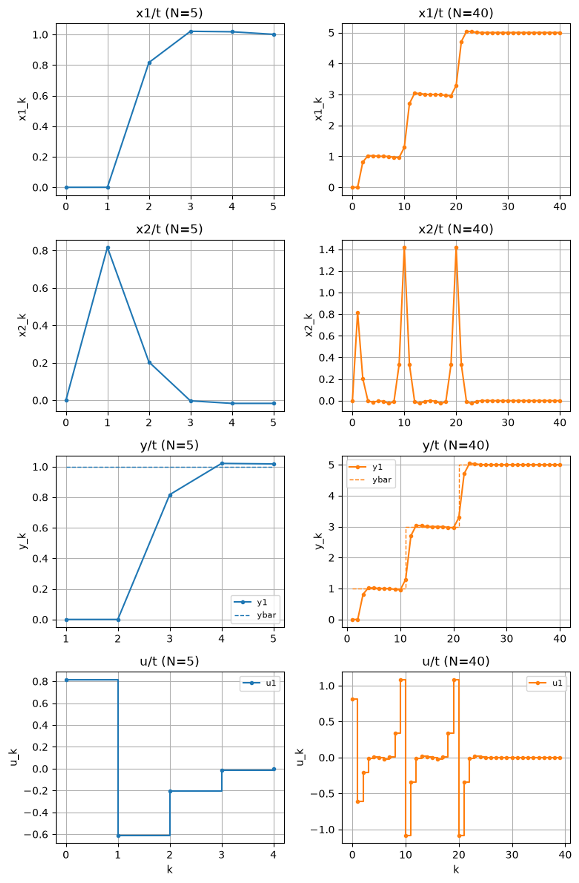
\includegraphics[width=0.85\textwidth]{graphics/LTI_Open_Loop_R0_1.png}
    \caption{Open-loop tracking performance for \(R=0.1\), Left-side is when N=5 with the averaged RMSE 0.450392, right-side is the case when N=40 with the averaged RMSE 0.172099}
    \label{fig:open_loop_R01}
\end{figure}


\subsubsection*{Case 2: \(R=0.5\)}


\begin{figure}[H]
    \centering
    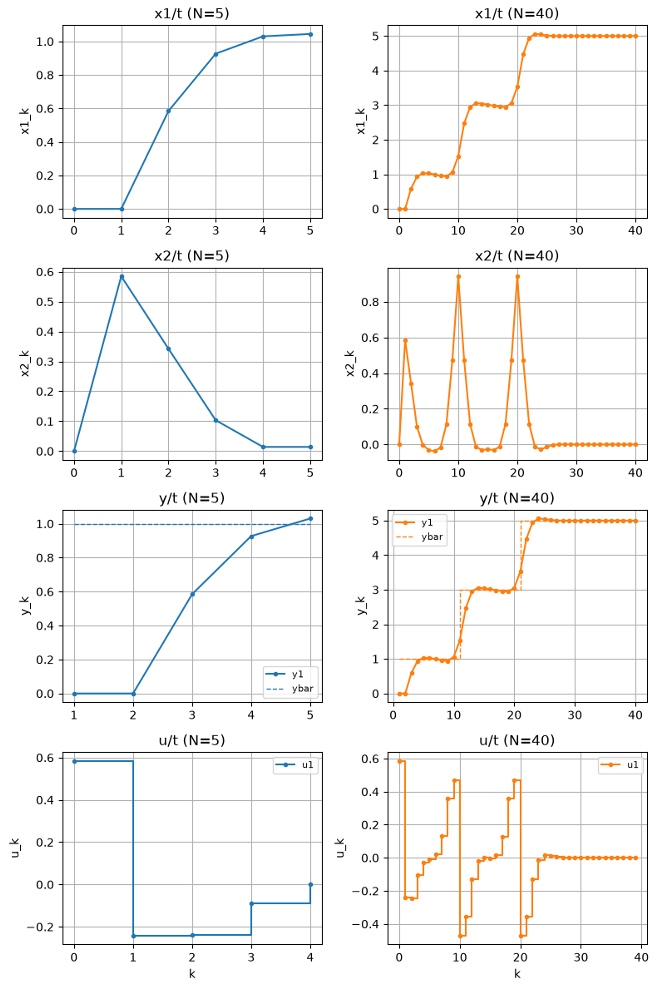
\includegraphics[width=0.85\textwidth]{graphics/LTI_Open_Loop_R0_5.png}
    \caption{Open-loop tracking performance for \(R=0.5\), Left-side is when N=5 with the averaged RMSE 0.469931, right-side is the case when N=40 with the averaged RMSE 0.220377}
    \label{fig:open_loop_R05}
\end{figure}


\subsubsection*{Case 3: \(R=5.0\)}


\begin{figure}[H]
    \centering
    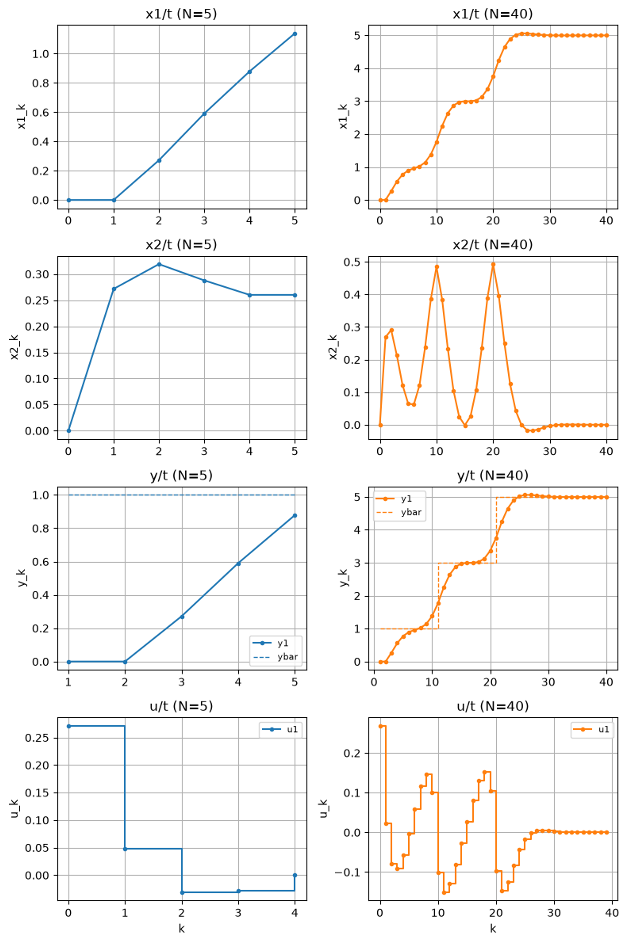
\includegraphics[width=0.85\textwidth]{graphics/LTI_Open_Loop_R5_0.png}
    \caption{Open-loop tracking performance for \(R=5.0\), Left-side is when N=5 with the averaged RMSE 0.571764, right-side is the case when N=40 with the averaged RMSE 0.344596}
    \label{fig:open_loop_R5}
\end{figure}

\subsubsection*{Comparison}

The results demonstrate the trade-off between reference tracking performance and control effort introduced by the weighting matrix \(R\). As the value of \(R\) increases, the contribution of the term \(U^TRU\) to the objective function becomes more significant. Consequently, the optimizer increasingly penalizes large control inputs and attempts to reduce the magnitude of \(U\).

For a small value such as \(R=0.1\), the controller is willing to use relatively large control actions in order to achieve accurate reference tracking. As \(R\) is increased to \(0.5\) and subsequently to \(5\), the control actions become less aggressive. The system therefore has increasing difficulty following changes in the reference trajectory, resulting in larger tracking errors.

Hence, increasing \(R\) improves the economy of the control action at the expense of tracking performance. The selection of \(R\) therefore represents a compromise between minimizing the control effort and maintaining accurate reference tracking.

\section{Closed-Loop Implementation}
\label{sec:closed_loop}

The open-loop implementation computes the optimal control sequence only once from the initial state and applies the complete sequence without further optimization. In contrast, the closed-loop implementation repeatedly solves the optimal control problem using the most recent state information.

This approach follows the receding-horizon principle. At each time step, a new optimal input sequence is calculated, but only its first control action is applied to the system. At the following time step, the state is updated and the optimization problem is solved again.

\subsection{Implementation Procedure}

The prediction horizon \(N\), control horizon \(N_c\), total simulation length \(N_{\mathrm{end}}\), reference trajectory, weighting matrices \(Q\) and \(R\), and initial state \(x_0\) are first specified.

The prediction and control horizons satisfy

\begin{equation}
    N_c \leq N
\end{equation}

The stacked prediction model derived previously is

\begin{equation}
    Y = \Phi x_k + \Gamma U_{\mathrm{full}},
    \label{eq:closed_loop_prediction}
\end{equation}

where

\begin{equation}
    \Phi =
    \begin{bmatrix}
        CA \\
        CA^2 \\
        \vdots \\
        CA^N
    \end{bmatrix}
\end{equation}

and

\begin{equation}
    \Gamma =
    \begin{bmatrix}
        CB & 0 & \cdots & 0 \\
        CAB & CB & \cdots & 0 \\
        \vdots & \vdots & \ddots & \vdots \\
        CA^{N-1}B & CA^{N-2}B & \cdots & CB
    \end{bmatrix}
\end{equation}

When a control horizon \(N_c\) shorter than the prediction horizon is used, the independent control variables are collected in

\begin{equation}
    U_c =
    \begin{bmatrix}
        u_0 \\
        u_1 \\
        \vdots \\
        u_{N_c-1}
    \end{bmatrix}
\end{equation}

The complete input sequence over the prediction horizon is then generated as

\begin{equation}
    U_{\mathrm{full}} = T U_c,
    \label{eq:closed_loop_control_mapping}
\end{equation}

where \(T\) is a control-horizon mapping matrix. This matrix maps the \(N_c\) independent control variables to the full prediction horizon.

Substituting \cref{eq:closed_loop_control_mapping} into the prediction model gives

\begin{equation}
    Y
    =
    \Phi x_k
    +
    \Gamma T U_c
    \label{eq:closed_loop_reduced_prediction}
\end{equation}

At each time step \(k\), the reference trajectory corresponding to the current prediction window is denoted by \(\bar{Y}_k\). The quadratic cost function is therefore written as

\begin{equation}
    \phi(U_c)
    =
    \left(
        \Phi x_k
        +
        \Gamma T U_c
        -
        \bar{Y}_k
    \right)^T
    Q
    \left(
        \Phi x_k
        +
        \Gamma T U_c
        -
        \bar{Y}_k
    \right)
    +
    U_c^T R U_c
    \label{eq:closed_loop_cost}
\end{equation}

The optimization problem is solved again at every sampling instant. Following the same derivation as in the previous section, the optimal control sequence becomes

\begin{equation}
    U_c^\ast
    =
    -
    \left[
        (\Gamma T)^T Q (\Gamma T) + R
    \right]^{-1}
    (\Gamma T)^T Q
    \left(
        \Phi x_k-\bar{Y}_k
    \right)
    \label{eq:closed_loop_optimal_u}
\end{equation}

Unlike the open-loop implementation, the complete optimal sequence is not applied to the system. Instead, only the first control input is selected.

A selection matrix \(\Pi\) can be defined such that

\begin{equation}
    u_k = \Pi U_c^\ast
    \label{eq:closed_loop_first_input}
\end{equation}

For a scalar-input system,

\begin{equation}
    \Pi =
    \begin{bmatrix}
        1 & 0 & \cdots & 0
    \end{bmatrix}
\end{equation}

The selected input is then applied to the system:

\begin{align}
    x_{k+1} &= Ax_k + Bu_k, \\
    y_k &= Cx_k
\end{align}

After obtaining the new state \(x_{k+1}\), the prediction window is shifted forward by one time step. The reference trajectory is updated accordingly, and the optimization problem is solved again.

This procedure is repeated until

\begin{equation}
    k = N_{\mathrm{end}}-1
\end{equation}

Therefore, the closed-loop algorithm can be summarized as follows:

\begin{enumerate}
    \item Select \(N\), \(N_c\), \(N_{\mathrm{end}}\), \(Q\), \(R\), the reference trajectory, and \(x_0\).
    \item Construct the prediction matrices \(\Phi\) and \(\Gamma\), together with the control-horizon mapping matrix \(T\).
    \item At time step \(k\), construct the reference vector \(\bar{Y}_k\) over the current prediction horizon.
    \item Compute the optimal control sequence \(U_c^\ast\).
    \item Apply only the first control action,
    \[
        u_k = \Pi U_c^\ast
    \]
    \item Update the system state and output.
    \item Shift the prediction horizon and repeat the optimization for \(k+1\).
\end{enumerate}

\newpage
\subsection{Results}
\label{subsec:closed_loop_results}

The closed-loop controller was evaluated using the same LTI system considered in the open-loop implementation:

\begin{equation}
    A =
    \begin{bmatrix}
        1 & 1 \\
        0 & 1
    \end{bmatrix},
    \qquad
    B =
    \begin{bmatrix}
        0 \\
        1
    \end{bmatrix},
    \qquad
    C =
    \begin{bmatrix}
        1 & 0
    \end{bmatrix}
\end{equation}

The reference output was chosen as

\begin{equation}
    \bar{y}
    =
    \begin{bmatrix}
        1.0 & 3.0 & 5.0
    \end{bmatrix},
\end{equation}

where the reference value changes every 10 simulation steps.

For this experiment, the control-input weighting was selected as

\begin{equation}
    R = 0.1
\end{equation}

Also, in our example, the prediction horizon is chosen to be the same as the control horizon. So,

\begin{equation}
    T = I,\quad
    U_{full}=U_c
\end{equation}

\begin{figure}[H]
    \centering
    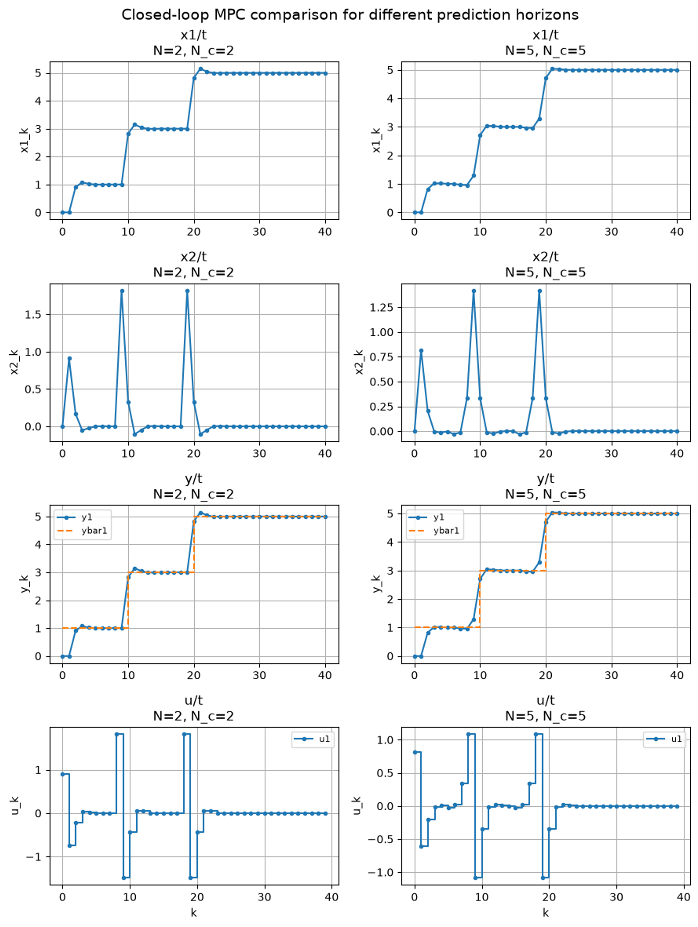
\includegraphics[width=0.85\textwidth]{graphics/LTI_Closed_Loop_R0_1.png}
    \caption{Closed-loop tracking performance for \(R=5.0\), Left-side is when N=2 with the averaged RMSE 0.238485, right-side is the case when N=5 with the averaged RMSE 0.242733}
    \label{fig:closed_loop_R01}
\end{figure}
